
%---------------------------------------------------------------------------%

\textbf{The Continuous Uniform Distribution}



\begin{center}
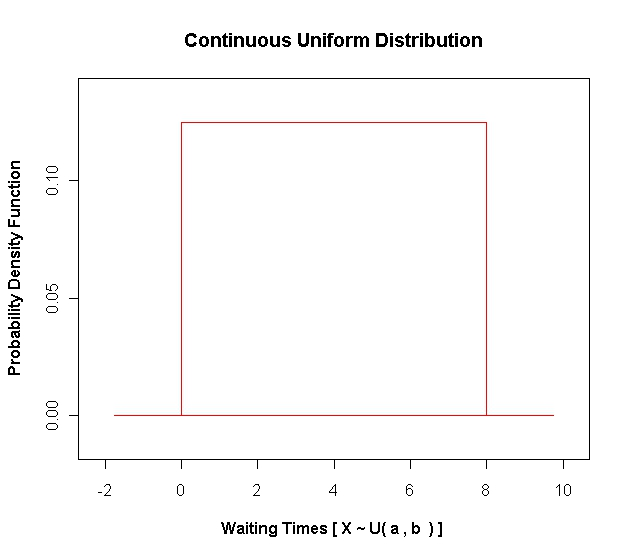
\includegraphics[scale=0.35]{images/6AUniform}

\end{center}
\medskip
%---------------------------------------------------------------------------%

%---------------------------------------------------------------------------------------------------------%
{
\textbf{Uniform Distribution: Cumulative Distribution}
\begin{itemize}

\item For any value ``c" between the minimum value a and the maximum
value $b$, we can say
\item $P(X \geq c)$ \[P(X \geq c) = {b-c \over b-a}\]
here $b$ is the upper bound while $c$ is the lower bound
\item $P(X \leq c)$ \[P(X \leq c) = {c-a \over b-a}\]
here $c$ is the upper bound while $a$ is the lower bound.
\end{itemize}
}

%-----------------------------------------------------------------------------%
{
\textbf{Uniform Distribution: Mean and Variance}
\begin{itemize}
\item The mean of the continuous uniform distribution, with parameters $a$ and $b$ is
\[ E(X) = {a+b \over 2}\]
\item The variance is computed as
\[ V(X) = {(b-a)^2 \over 12}\]
\end{itemize}
}
